% Conditioning as Group Action. ICLR layout is EMULATED here (times, 10pt, 1in margins, review
% header): drop in the official iclr20XX_conference.sty at submission time, which is a one-line
% preamble swap.
% Tables/figures AUTO-GENERATED from results/*.json (gen_tables.py, figures.py) — never hand-edit.
% Prose register: paper-writing skill (plain words, claim-first, active voice, no em-dashes).
\documentclass[10pt,letterpaper]{article}
\usepackage[margin=1in]{geometry}
\usepackage{amsmath,amsthm}
\usepackage{newtxtext,newtxmath}
\usepackage{graphicx,booktabs}
\usepackage[numbers,sort&compress]{natbib}
\usepackage[colorlinks,citecolor=blue,linkcolor=blue,urlcolor=blue]{hyperref}
\usepackage{microtype,fancyhdr}
\pagestyle{fancy}\fancyhf{}\fancyhead[L]{\footnotesize Under review as a conference paper at ICLR 2027}
\fancyfoot[C]{\thepage}\renewcommand{\headrulewidth}{0.4pt}
\newtheorem{proposition}{Proposition}
\newtheorem{definition}{Definition}
\newcommand{\T}{T}

\title{Conditioning as Group Action:\\ Exact Compositional Conditioning at FiLM Cost}
\author{Anonymous authors\\ Paper under double-blind review}
\date{}

\begin{document}
\maketitle

\begin{abstract}
Networks are conditioned by scaling features (FiLM) or by generating weights (hypernetworks).
Both learn what each condition does. Neither learns what two conditions do together unless
training data shows them together. We condition by rotating features, with rotation angles a
linear function of the condition. Rotations add, so combined conditions compose automatically,
and the network handles combinations it never saw. \textbf{CGA} (Conditioning as Group Action)
formalizes this: the condition enters the operator linearly in an abelian Lie algebra,
$\T(c)=P\exp(\mathrm{A}(Wc))P^{\top}$, so $\T(c_1{+}c_2)=\T(c_1)\T(c_2)$ holds for any weights.
A diagonal algebra yields a compositional FiLM variant; the rotation algebra with scalar
position is RoPE. Under a pre-registered protocol (margins, tests, and splits committed before
every run; conditioning cost within $1.2\times$ FiLM), CGA posts the lowest error on
never-trained condition combinations across five transformation suites, with complete seed
separation ($p{=}9.1{\times}10^{-5}$, $N{=}10$) and zero-shot extrapolation to combinations
longer than any trained. Swapping its linear map for an MLP raises error up to
$4.3{\times}10^{4}$; the most expressive baselines generalize worst. Three registered gates
returned negatives that bound the method: a fit penalty on rich scenes, a content-conditioning
failure (rotations move information and cannot add it), and rollouts limited by representation
consistency. The negatives specify the successor. \textbf{Complex FiLM}, magnitude for content
and phase for composition, beats FiLM by 36\% on unseen combinations and matches it on content
($0.97\times$) under two further pre-registered gates. The same structure yields guidance
without classifier-free extrapolation: powering the condition distorts $2$--$5\times$ less than
CFG at every strength, with no second forward pass. One operator, both roles, FiLM cost.
\end{abstract}

\section{Introduction}

Conditioning, injecting a class, an action, a timestep, or a text embedding into a network's
computation, recurs in nearly every conditional model. Diffusion models modulate every block on
the timestep and class via adaLN \citep{peebles2023dit}; visual reasoning, speech, and RL
systems modulate features on questions, speakers, and goals \citep{perez2018film}; world models
condition latent dynamics on actions. Almost all of this conditioning is carried by three
mechanisms: concatenation, feature-wise affine modulation (FiLM), or a hypernetwork that emits
weights from the condition.

These mechanisms sit at two extremes of an expressivity axis. FiLM's diagonal transform is
cheap and stable but cannot mix features. Hypernetworks can express any linear operator but pay
quadratic cost and, as we show, memorize the training conditions: their error on unseen
combinations of familiar conditions is worse than FiLM's, despite 43$\times$ the conditioning
compute. The middle of this axis, structured operator families between diagonal and dense, is
well explored for weight fine-tuning \citep{hu2022lora,qiu2023oft,liu2024boft,yuan2024hra} and
largely unexplored in FiLM's role: per-sample, input-conditioned modulation of activations.

We ask which structure, at FiLM-level cost, buys compositional generalization: correct behavior
on combinations of conditions never seen together in training. Our answer imports a mechanism
from positional encoding. RoPE \citep{su2021rope} and its generalization GRAPE \citep{grape2025}
encode position $n$ as a group action $G(n)=\exp(n\,\omega L)$; because position enters linearly
in the Lie algebra, $G(n{+}m)=G(n)G(m)$ holds exactly. We transplant this construction from
scalar positions in attention to arbitrary condition vectors in activation modulation.

\paragraph{Contributions.}
\textbf{(1) Framework.} CGA treats conditioning as a group representation of the condition
space; FiLM, RoPE, and GRAPE drop out as special cases, and a two-line proposition makes
condition composition exact for any weights (\S\ref{sec:framework}).
\textbf{(2) Protocol.} A pre-registered, budget-fair evaluation: margins, statistical tests, and
single-read splits committed to version control before every run, with a shared counter
enforcing parameter and FLOP parity; we report every verdict, including negatives against our
own predictions (\S\ref{sec:protocol}).
\textbf{(3) Where it works, and where it stops.} Five confirmations where conditions are
transformations, by up to five orders of magnitude, including the finding that more expressive
conditioners generalize worse in every image suite; and three negatives with mechanisms (fit,
content, rollouts) that say exactly where the guarantee stops paying
(\S\ref{sec:results}).
\textbf{(4) Successor and guidance.} The negatives specify Complex FiLM, validated under two
further gates as a FiLM replacement covering both conditioning roles, whose phase channel also
yields guidance as an exact operator power: $2$--$5\times$ less distortion than CFG with no
unconditional pass (\S\ref{sec:results}).

\section{Related work}
\label{sec:related}

\paragraph{FiLM and conditional normalization.} FiLM \citep{perez2018film} and its normalized
variants (conditional BN/LN, adaLN in DiT \citep{peebles2023dit}) apply per-feature affine
transforms generated from a condition. All are diagonal. We keep FiLM's role and enrich only
the operator.

\paragraph{Structured operators in PEFT.} Low-rank, orthogonal, and butterfly operator families
are well studied as weight fine-tuning: LoRA \citep{hu2022lora}, OFT \citep{qiu2023oft}, BOFT
\citep{liu2024boft}, HRA \citep{yuan2024hra}, Group-and-Shuffle \citep{gorbunov2024gs};
\citet{he2022unified} give a unified view. These learn one fixed transform per task. Our
setting differs on every axis that matters: per-sample, input-conditioned, activation-space,
and evaluated for compositional generalization. Hypernetworks \citep{ha2017hypernetworks}
generate weights from conditions and inherit the memorization behavior we quantify.

\paragraph{Position encodings as group actions.} RoPE \citep{su2021rope} rotates query-key
pairs by angles linear in position; GRAPE \citep{grape2025} generalizes this to group
representations with exact relative laws. The mechanism is theirs; our contribution is the
transplant to arbitrary condition vectors in FiLM's role, with a learned basis, and the
budget-fair compositional evidence.

\paragraph{Compositional generation.} \citet{montero2021role} showed reconstruction-trained
generative models fail on unseen factor combinations. Score and energy composition
\citep{liu2022composable} composes concepts across separate conditional passes; we compose
conditions inside the operator, in one pass. Symmetry-based representation learning
\citep{higgins2018towards,cohen2016group} argues latents should carry group actions; we supply
the conditioning-side mechanism.

\paragraph{Nearest prior work, found adversarially.} Feature-space rotations with exact
composition exist for geometric transformations \citep{worrall2017}; abelian exponential-map
operators for disentanglement \citep{zhu2021clgvae}; attribute operators for recognition
\citep{nagarajan2018attrop}; multilinear attribute mixing for unseen combinations
\citep{georgopoulos2020}; per-sample amplitude-and-phase activation modulation in periodic
implicit networks \citep{chan2021pigan}; and composition by complex phase addition in
knowledge-graph embeddings \citep{sun2019rotate}. Rotation-structured latent world models with
latent-prediction losses originate with \citet{quessard2020}, \citet{caselles2019}, and the
homomorphism autoencoder \citep{keurti2023}, whose composition property is emergent rather than
imposed; latent consistency objectives are standard in model-based RL \citep{hansen2022tdmpc}.
Guidance has been moved into the conditioning path by distilling a CFG teacher
\citep{fu2025teefusion}, and CFG's high-scale distortion is established
\citep{bradley2024cfg}. We claim none of these components. We claim the combination: a
group-structured operator in FiLM's role at budget parity, composition imposed exactly by a
linear-in-algebra map, magnitude split from phase as content and composition channels, guidance
as an exact power, and verdicts from pre-registered gates.

\section{The CGA framework}
\label{sec:framework}

Let $x\in\mathbb{R}^d$ be features and $c\in\mathbb{R}^k$ a condition. FiLM computes
$y=\gamma(c)\odot x+\beta(c)$; hypernetworks emit $W(c)$. All are instances of
\begin{equation}
y=\T(c)\,x+\beta(c),
\label{eq:family}
\end{equation}
and they differ only in where the per-sample operator $\T(c)$ comes from.

\begin{definition}[Compositional conditioner]
$\T:\mathbb{R}^k\!\to\!\mathrm{GL}(d)$ is \emph{compositional} if it is a homomorphism from
$(\mathbb{R}^k,+)$: $\T(c_1{+}c_2)=\T(c_1)\,\T(c_2)$ and $\T(0)=I$.
\end{definition}

\begin{proposition}[Exact composition by construction]
\label{prop:main}
Let $\mathfrak{a}$ be an abelian subalgebra of $\mathfrak{gl}(d)$, $\mathrm{A}:\mathbb{R}^m\!\to\!
\mathfrak{a}$ linear, $W\in\mathbb{R}^{m\times k}$, and $P$ orthogonal. Then
$\T(c)=P\exp(\mathrm{A}(Wc))\,P^{\top}$ is a compositional conditioner for every $W,P$. If
$\mathfrak{a}$ is skew-symmetric, $\T(c)$ is orthogonal.
\end{proposition}
\begin{proof}
$\exp(X)\exp(Y)=\exp(X{+}Y)$ for commuting $X,Y$; $\mathrm{A}\circ W$ is linear; conjugation
preserves products; $\exp(0)=I$.
\end{proof}

Composition is usually a behavior the network must learn from data. Here it is a property of
the parametrization. It holds at initialization, during training, and far outside the training
distribution. Training only decides which directions the condition rotates and how fast.

\paragraph{Special cases.} Choices of $(\mathfrak{a}, c, P)$ recover deployed mechanisms:

\begin{center}
\small
\begin{tabular}{llll}
\toprule
$\mathfrak{a}$ & condition & $P$ & recovered mechanism \\
\midrule
$\mathrm{diag}(\mathbb{R}^d)$ & $c$ & $I$ & \emph{exponential FiLM}: $y=e^{Wc}\odot x$ (compositional) \\
$\mathfrak{so}(2)^{d/2}$ & $c=n$ (scalar position) & $I$ & RoPE \citep{su2021rope} \\
$\mathfrak{so}(2)^{d/2}$ & $c=n$, learned planes & learned & multiplicative GRAPE \citep{grape2025} \\
$\mathfrak{so}(2)^{d/2}$ & general $c\in\mathbb{R}^k$ & structured & \textbf{this work} (FiLM's role) \\
$\mathrm{diag} \times \mathfrak{so}(2)^{d/2}$ & general $c$ & canonical & \textbf{Complex FiLM} (\S\ref{sec:results}) \\
\bottomrule
\end{tabular}
\end{center}

Standard FiLM reaches the same diagonal operators through an MLP head $\gamma(c)$. The
operators match; the composition law is missing, and \S\ref{sec:results} shows the missing law
is exactly what fails on unseen combinations.

\paragraph{Cost.}
With $\mathfrak{a}=\mathfrak{so}(2)^{d/2}$, $\exp$ is closed-form planar rotation: $3d$ FLOPs,
no matrix exponential. The basis $P$ is the whole budget question. A dense learned $P$ costs
$4d^2$ FLOPs per sample, which is $1.52\times$ FiLM's entire conditioning path at $d{=}128$.
Two fixes work. A structured orthogonal $P$ (five block-diagonal Cayley layers with fixed
shuffles, following Group-and-Shuffle) brings the total to $1.11\times$ FiLM, with 4{,}800
parameters against the 8{,}128 dimensions of $\mathrm{SO}(128)$; that is enough, because $P$
only needs the planes the condition acts on. Inside a transformer, no explicit $P$ is needed:
the adjacent dense projections absorb the basis, which is how RoPE deploys. The operator equals
the identity at initialization and at $c{=}0$, and every singular value is 1. Unit tests pin
all three properties. Complex FiLM extends the algebra to $\mathrm{diag}\times
\mathfrak{so}(2)^{d/2}$: each feature pair is multiplied by $m\,e^{i\theta}$, with magnitude
from FiLM's expressive head (the content channel) and phase linear in the condition (the
composition channel), at $0.84\times$ FiLM's cost in our harnesses.

\section{Pre-registered, budget-fair protocol}
\label{sec:protocol}

\paragraph{Design.} Every suite is pre-registered: success margins, statistical tests
($N{=}10$ seeds, one-sided Mann--Whitney $p\le0.01$, Cliff's $|\delta|\ge0.474$), and data
splits were fixed and committed to version control before each run. Each test split is read
once, after all selection on a validation split. All arms share one backbone and one training
recipe. A shared counter enforces the budget: our conditioning path stays within $1.20\times$
FiLM's FLOPs and $1.05\times$ the smallest hypernetwork baseline's parameters; baselines may be
larger, and reach $48\times$ our parameter count. Deviations are dated amendments in the
committed specifications, plus one accounting erratum that our own audit caught and that
downgraded a favorable verdict.

\paragraph{Threats to validity, and the design answer.} The benchmarks are self-constructed,
so we built them to remove judgment from scoring: dSprites and 3D~Shapes are deterministic
factor-to-image maps, so every held-out condition has a unique ground-truth image and pixel
error is an objective compositional metric, with no perceptual score and no human rating.
Pre-registration removes outcome-contingent analysis; the verdicts below include three
negatives, one of which falsified our own headline prediction. Every number in this paper
regenerates from committed logs with one command per suite, so replication at our scale costs
one training run.

\paragraph{Arms.} FiLM; conditional LayerNorm; Concat-MLP; a dense hypernetwork
$I{+}\Delta W(c)$; a dynamic low-rank map $I{+}A(c)B(c)^{\top}$; the Lie operator; Complex FiLM
(both variants); and an MLP-head ablation of our own method (same basis, same operator family,
more compute, no linearity).

\paragraph{Suites.} \textbf{S1/S2 (synthetic):} learn $y=M(c)x$, where $c$ selects a
combination of 8 rotation primitives; S2 hides the primitives behind a random basis and tests
all 56 never-trained \emph{triples}. \textbf{S3/S3b (dSprites) and S4 (3D~Shapes):} image
transformation: encode a real image, apply $\T(\Delta)$ on the learned latent for a factor
change $\Delta$, decode, and score pixel error against the true transformed image; OOD means
never-trained \emph{types} of two-factor changes; S3b/S4 add a categorical shape factor.
\textbf{S5 (content):} a small diffusion transformer generates dSprites images from full factor
specifications. \textbf{S6 (rollouts):} a world model applies the conditioning arm recurrently,
one action per step; horizons 10 and 20 after training on 3. \textbf{S7 (successor):} Complex
FiLM through the S3 and S5 harnesses. \textbf{S8 (guidance):} condition-dropout training, then
CFG at strength $w$ for FiLM against condition powering for Complex FiLM, scored against
deterministic ground truth per strength.

\section{Results}
\label{sec:results}

\begin{table}[t]
\centering
\caption{Error on never-trained condition combinations: mean (seed sd) over 10 seeds. CGA is
lowest in every column, with complete seed separation against the strongest hypernetwork
baseline ($p{=}9.1{\times}10^{-5}$, $\delta{=}{-}1.0$). S1--S3b pass the full pre-registered
gate; S4 fails a separate fit criterion (text). S7 is the Complex FiLM rerun of the S3 harness.}
\label{tab:main}
\small
% AUTO-GENERATED by gen_tables.py — do not edit
\begin{tabular}{lcccccc}
\toprule
Conditioner & S1 & S2 & S3 & S3b & S4 & S7 \\
\midrule
FiLM & $1.3\,(0.1)\!\times\!10^{-2}$ & $1.6\,(0.04)\!\times\!10^{-2}$ & $3.0\,(0.2)\!\times\!10^{-3}$ & $5.9\,(0.2)\!\times\!10^{-3}$ & $4.5\,(1.0)\!\times\!10^{-3}$ & $3.1\,(0.2)\!\times\!10^{-3}$ \\
Concat-MLP & $1.5\,(0.3)\!\times\!10^{-2}$ & $1.1\,(0.4)\!\times\!10^{-2}$ & $2.9\,(0.1)\!\times\!10^{-3}$ & $6.3\,(0.2)\!\times\!10^{-3}$ & $5.4\,(5.2)\!\times\!10^{-3}$ & -- \\
Cond-LN & $2.4\,(0.1)\!\times\!10^{-2}$ & $2.7\,(0.05)\!\times\!10^{-2}$ & $3.2\,(0.2)\!\times\!10^{-3}$ & $6.1\,(0.3)\!\times\!10^{-3}$ & $8.6\,(13.1)\!\times\!10^{-3}$ & -- \\
Hypernetwork & $1.9\,(0.3)\!\times\!10^{-3}$ & $3.4\,(0.9)\!\times\!10^{-3}$ & $3.8\,(0.3)\!\times\!10^{-3}$ & $7.0\,(0.4)\!\times\!10^{-3}$ & $9.3\,(2.3)\!\times\!10^{-3}$ & $3.8\,(0.2)\!\times\!10^{-3}$ \\
Dyn.\ low-rank & $5.7\,(0.5)\!\times\!10^{-3}$ & $6.1\,(0.4)\!\times\!10^{-3}$ & $5.1\,(0.9)\!\times\!10^{-3}$ & $8.1\,(0.4)\!\times\!10^{-3}$ & $2.0\,(0.4)\!\times\!10^{-2}$ & -- \\
MLP-head (abl.) & -- & $1.1\,(0.2)\!\times\!10^{-3}$ & $2.7\,(0.2)\!\times\!10^{-3}$ & $5.0\,(0.2)\!\times\!10^{-3}$ & $3.3\,(0.8)\!\times\!10^{-3}$ & -- \\
Complex FiLM (lin.) & -- & -- & -- & -- & -- & $2.0\,(0.1)\!\times\!10^{-3}$ \\
\textbf{Complex FiLM} & -- & -- & -- & -- & -- & $2.0\,(0.2)\!\times\!10^{-3}$ \\
\textbf{Lie (ours)} & $7.4\,(2.0)\!\times\!10^{-4}$ & $3.3\,(2.2)\!\times\!10^{-8}$ & $1.8\,(0.1)\!\times\!10^{-3}$ & $4.0\,(0.1)\!\times\!10^{-3}$ & $1.2\,(0.2)\!\times\!10^{-3}$ & $1.8\,(0.1)\!\times\!10^{-3}$ \\
\bottomrule
\end{tabular}
% gate margins: S1: 62\% vs.\ hypernet ($p=9e-5$); S2: 100\% vs.\ hypernet ($p=9e-5$); S3: 54\% vs.\ hypernet ($p=9e-5$); S3b: 43\% vs.\ hypernet ($p=9e-5$); S4: 87\% vs.\ hypernet ($p=9e-5$); S7: 0\% vs.\ ? ($p=0e+00$)

\end{table}

\begin{figure}[t]
\centering
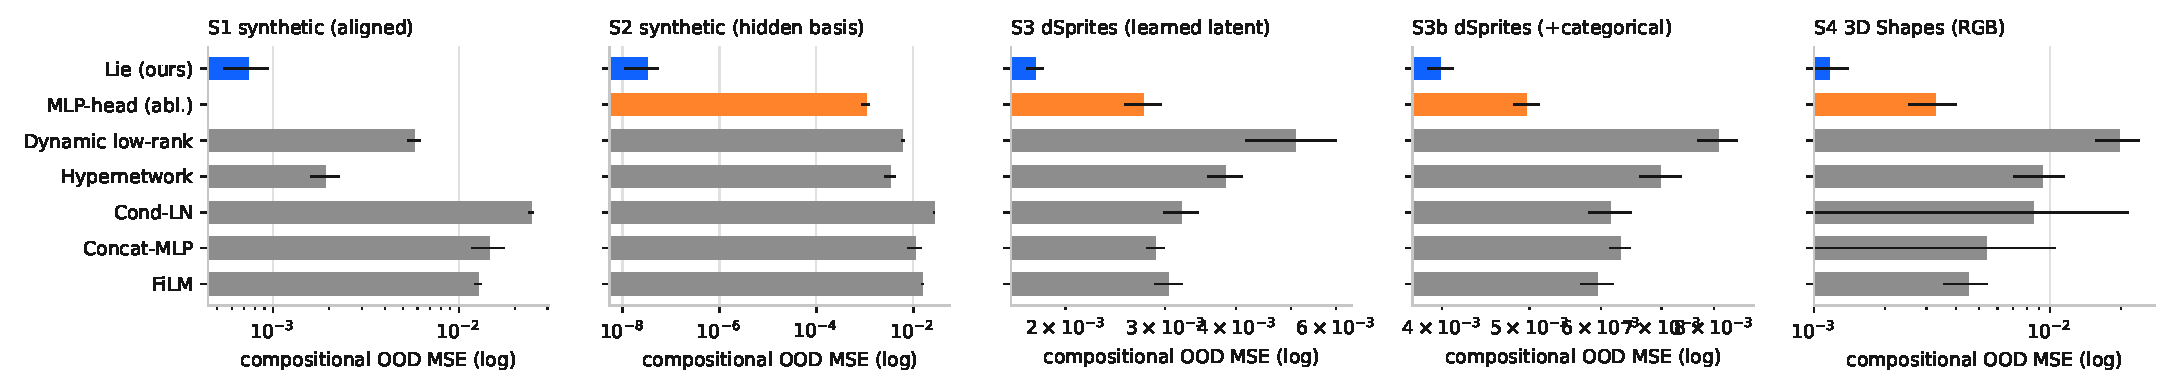
\includegraphics[width=\textwidth]{figs/f1_ood_all_stages.pdf}
\caption{Error on unseen condition combinations by conditioner (log scale; blue = ours, orange
= MLP-head ablation), across the five transformation suites.}
\label{fig:main}
\end{figure}

\begin{figure}[t]
\centering
\begin{minipage}[t]{0.55\textwidth}
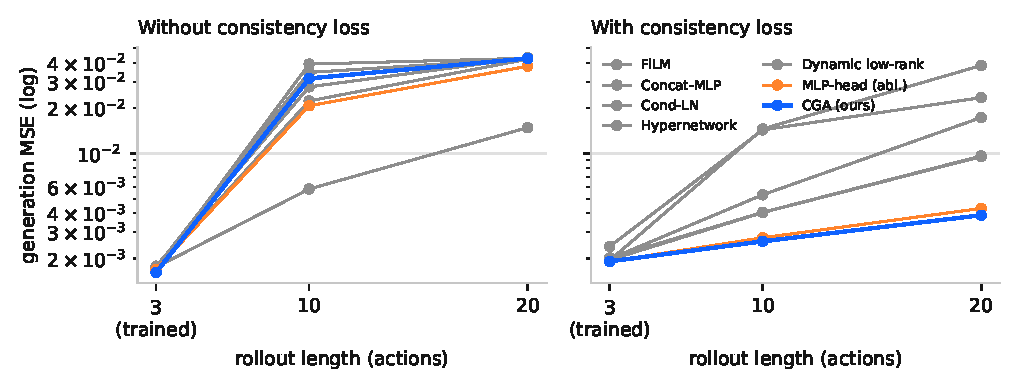
\includegraphics[width=\textwidth]{figs/f5_rollout_horizon.pdf}
\end{minipage}\hfill
\begin{minipage}[t]{0.42\textwidth}
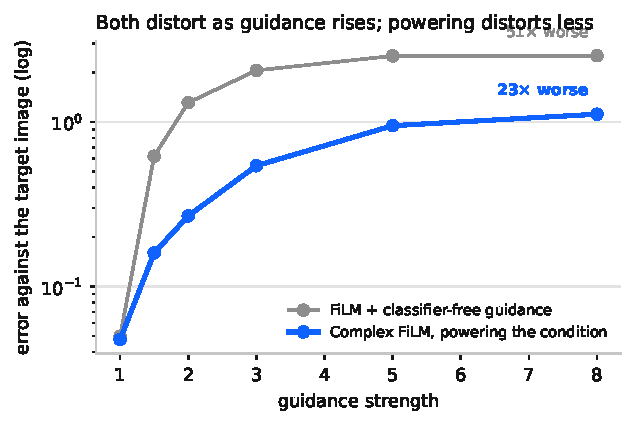
\includegraphics[width=\textwidth]{figs/f6_guidance_distortion.pdf}
\end{minipage}
\caption{\textbf{Left (S6/S6$'$):} rollout error versus horizon, without and with the
latent-consistency loss; with it, the isometric operator stays flat where every baseline
drifts. \textbf{Right (S8):} generation error versus guidance strength; CFG's linear
extrapolation distorts $50.7\times$ from strength 1 to 8, condition powering $23.7\times$,
staying $2$--$5\times$ lower throughout.}
\label{fig:horizon}
\end{figure}

\paragraph{(1) When conditions form a group, composition is solved.} On S2, CGA reaches
$3.3{\times}10^{-8}$ error on unseen pairs and $5.3{\times}10^{-8}$ on never-trained triples;
the best baseline sits five orders of magnitude higher and every baseline degrades as
combinations lengthen. Learned angles match the true generators to $2{\times}10^{-4}$ rad: reading the weights tells
you which plane each condition rotates, and how fast (Figure~\ref{fig:mech}).

\paragraph{(2) The advantage survives learned representations.} On dSprites every arm fits the
training distribution equally well, isolating composition. CGA's error grows $1.25\times$ from
training to unseen combinations ($1.63\times$ with the categorical factor); every baseline
grows $2.1$--$3.3\times$. CGA beats the strongest baseline by $53.8\%$ ($42.9\%$) at $39\times$
fewer conditioning FLOPs.

\paragraph{(3) The linear map is the mechanism.} The ablation keeps the basis and the operator
family, spends more compute, and swaps only the linear map for an MLP. It loses by
$4.3{\times}10^{4}\times$ on synthetic triples and $1.55\times$ on dSprites.

\paragraph{(4) More capacity makes it worse.} The two hypernetwork arms can express any
operator. They post the worst generalization gaps on images ($2.7$--$26\times$); their capacity
memorizes the training combinations.

\paragraph{(5) Three negatives, scored by the criteria we registered in advance.} On 3D~Shapes, CGA has the best OOD numbers
($87.5\%$ margin) but fits training $1.46\times$ worse than the best memorizer, tripping our
no-regression gate. In the content suite, rotation conditioning fails ($0.31$ vs.\ film's
$0.04$) and the ablation fails identically: a rotation moves information and cannot add any,
so it cannot carry ``generate this image.'' In the rollout suite, every arm compounds error at
the same rate; each step adds a small mismatch between predicted and true latent, which a
contraction shrinks and an isometry carries forever.

\paragraph{(6) A consistency loss completes the rollout recipe.} Training with
$\lambda\|\T(a)z_s-z_{s+1}\|^2$, applied to every arm equally, inverts the picture: the
rotation operator's horizon-20 error goes flat at $0.0039$ (growth $2.0\times$) against the
hypernetwork's $0.038$ (growth $19.8\times$) and FiLM's $0.017$ (Figure~\ref{fig:horizon},
left). The loss is standard in model-based RL \citep{hansen2022tdmpc}, and rotation transitions
with latent-prediction objectives appear in the homomorphism autoencoder \citep{keurti2023};
our contribution is the controlled decomposition at matched budget, plus a null result that sharpens
it: fixed uniform contraction at any rate from $0.003$ to $0.1$ leaves horizon-20 error
unchanged, so the correction must be adaptive. That suite's gate still returns a negative,
because a separate single-step criterion fails, and we report the suite that way.

\paragraph{(7) The negatives specify the fix, and it works.} Complex FiLM multiplies feature
pairs by $m\,e^{i\theta}$. Under two pre-registered gates it beats FiLM by $36\%$ on unseen
change types at fit parity and $0.84\times$ FiLM's cost, and matches FiLM on content generation
at $0.97\times$ its error (pre-registered non-inferiority margin $1.10\times$), where the pure
rotation failed by $7\times$. A linear magnitude channel fails ($0.19$): content needs the
expressive head. FiLM is the real part of the working operator; the whole complex number does
both jobs.

\paragraph{(8) Guidance without the second pass.} CFG's distortion at high scales is
established \citep{bradley2024cfg}; our benchmark isolates it against an exact
alternative, because the conditioning target is deterministic. CFG's error grows $50.7\times$ from strength 1 to 8; powering the condition
through the phase channel grows $23.7\times$ ($p{=}1.6{\times}10^{-4}$), stays $2$--$5\times$
lower at every strength above 1, matches at native strength ($0.96\times$), and needs no
unconditional pass and no distillation \citep{fu2025teefusion}
(Figure~\ref{fig:horizon}, right). Neither method improves over strength 1 here: the target is
deterministic, so there is no distribution to sharpen, exactly as the suite's registered caveat
stated.

\begin{figure}[t]
\centering
\begin{minipage}[t]{0.5\textwidth}
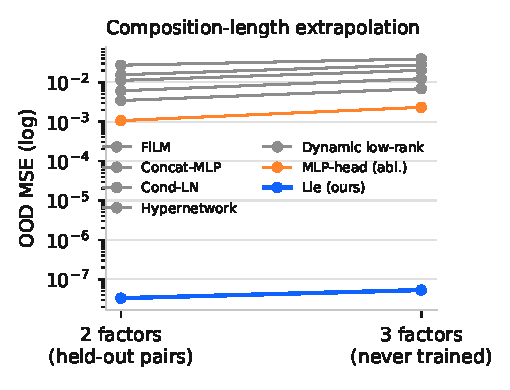
\includegraphics[width=\textwidth]{figs/f2_length_extrapolation.pdf}
\end{minipage}\hfill
\begin{minipage}[t]{0.4\textwidth}
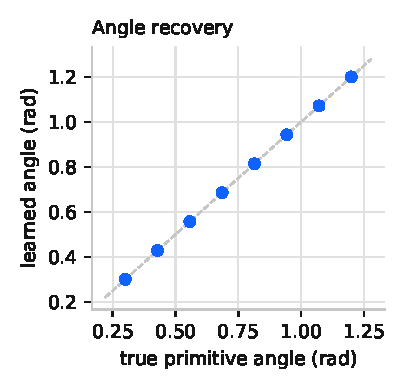
\includegraphics[width=\textwidth]{figs/f4_angle_recovery.pdf}
\end{minipage}
\caption{\textbf{Left (S2):} extrapolation to composition length 3, never trained; ours is
flat at $10^{-8}$ and every baseline degrades. \textbf{Right (S1):} learned singleton angles
recover the true generators to $2\times10^{-4}$ rad.}
\label{fig:mech}
\end{figure}

\section{Practical guidance}
\label{sec:practical}

Three rules for practitioners, from the eight suites.
\textbf{Use phase conditioning when your conditions are changes that combine.} Edit deltas,
attribute offsets, pose or camera adjustments, applied once. Cost matches FiLM, fit matches,
and behavior on never-trained combinations is $43\%$ to $10^5\times$ better; FiLM's failure
there is silent, and the guarantee removes that failure class.
\textbf{For conditions that say what to generate, use Complex FiLM or keep FiLM.} Pure rotation
fails there ($7\times$); Complex FiLM matches FiLM on content ($0.97\times$) while keeping the
composition wins, so it is the candidate drop-in at our evidence scale.
\textbf{In rollouts, pair an isometric operator with a consistency loss.} Without the loss, all
conditioners compound error at the same rate; with it, the rotation operator stays flat where
FiLM grows $4.5\times$ and a hypernetwork $10\times$.

\section{Limitations}
\label{sec:limits}

All evidence comes from controlled $64{\times}64$ benchmarks with known factors, width-128
models, and a single conditioning site; nothing here is validated at production scale, and the
natural deployment experiment is the adaLN site of a text-conditioned diffusion transformer.
Learned latents do not support exact group action: the real-image advantage is a reliable
$2\times$, not the synthetic $10^5\times$. S4 shows orthogonality can cost in-distribution fit
on rich scenes. The guidance benchmark measures distortion only, and cannot measure the
distribution-sharpening benefit CFG provides when the target is multimodal. Conditions far from any
group action, such as open-ended text, remain untested; the learned-condition-geometry
extension is future work.

\paragraph{Reproducibility statement.} We release the code, the pre-registrations, and the raw
logs. Every suite has a specification committed before its decision run; a registry maps each
suite label in this paper to the module that produced it, the log it wrote, and its verdict, so
a replicator reproduces any row with a single command. Every number, table, and figure here
regenerates from those append-only logs. Unit tests pin the operator invariants (identity at
initialization and at $c=0$, orthogonality, exact composition), the budget counters, and the
registry itself. All amendments and one accounting erratum, a FLOP undercount our own audit
caught that downgraded a favorable verdict, are disclosed with the results.

\begin{thebibliography}{30}
\bibitem[Perez et al.(2018)]{perez2018film} E.~Perez, F.~Strub, H.~de~Vries, V.~Dumoulin,
A.~Courville. FiLM: Visual reasoning with a general conditioning layer. \emph{AAAI}, 2018.
\bibitem[Peebles and Xie(2023)]{peebles2023dit} W.~Peebles, S.~Xie. Scalable diffusion models
with transformers. \emph{ICCV}, 2023.
\bibitem[Ha et al.(2017)]{ha2017hypernetworks} D.~Ha, A.~Dai, Q.~Le. Hypernetworks. \emph{ICLR},
2017.
\bibitem[Su et al.(2021)]{su2021rope} J.~Su, Y.~Lu, S.~Pan, A.~Murtadha, B.~Wen, Y.~Liu.
RoFormer: Enhanced transformer with rotary position embedding. \emph{arXiv:2104.09864}, 2021.
\bibitem[GRAPE(2026)]{grape2025} L.~Zhang, K.~Chen, X.~Liu, et~al. Group representational
position encoding. \emph{ICLR}, 2026.
\bibitem[Hu et al.(2022)]{hu2022lora} E.~Hu et al. LoRA: Low-rank adaptation of large language
models. \emph{ICLR}, 2022.
\bibitem[Qiu et al.(2023)]{qiu2023oft} Z.~Qiu et al. Controlling text-to-image diffusion by
orthogonal finetuning. \emph{NeurIPS}, 2023.
\bibitem[Liu et al.(2024)]{liu2024boft} W.~Liu et al. Parameter-efficient orthogonal finetuning
via butterfly factorization. \emph{ICLR}, 2024.
\bibitem[Yuan et al.(2024)]{yuan2024hra} S.~Yuan, H.~Liu, H.~Xu. Householder reflection
adaptation. \emph{NeurIPS}, 2024.
\bibitem[Gorbunov et al.(2024)]{gorbunov2024gs} M.~Gorbunov et al. Group and shuffle: Efficient
structured orthogonal parametrization. \emph{NeurIPS}, 2024.
\bibitem[He et al.(2022)]{he2022unified} J.~He, C.~Zhou, X.~Ma, T.~Berg-Kirkpatrick, G.~Neubig.
Towards a unified view of parameter-efficient transfer learning. \emph{ICLR}, 2022.
\bibitem[Montero et al.(2021)]{montero2021role} M.~Montero, C.~Ludwig, R.~Costa, G.~Malhotra,
J.~Bowers. The role of disentanglement in generalisation. \emph{ICLR}, 2021.
\bibitem[Higgins et al.(2018)]{higgins2018towards} I.~Higgins et al. Towards a definition of
disentangled representations. \emph{arXiv:1812.02230}, 2018.
\bibitem[Cohen and Welling(2016)]{cohen2016group} T.~Cohen, M.~Welling. Group equivariant
convolutional networks. \emph{ICML}, 2016.
\bibitem[Quessard et al.(2020)]{quessard2020} R.~Quessard, T.~Barrett, W.~Clements. Learning
disentangled representations and group structure of dynamical environments. \emph{NeurIPS},
2020.
\bibitem[Caselles-Dupr\'e et al.(2019)]{caselles2019} H.~Caselles-Dupr\'e, M.~Garcia-Ortiz,
D.~Filliat. Symmetry-based disentangled representation learning requires interaction with
environments. \emph{NeurIPS}, 2019.
\bibitem[Worrall et al.(2017)]{worrall2017} D.~Worrall, S.~Garbin, D.~Turmukhambetov,
G.~Brostow. Interpretable transformations with encoder-decoder networks. \emph{ICCV}, 2017.
\bibitem[Keurti et al.(2023)]{keurti2023} H.~Keurti, A.~Neitz, S.~Weichwald, B.~Sch\"olkopf,
et~al. Homomorphism autoencoder: Learning group structured representations from observed
transitions. \emph{ICML}, 2023.
\bibitem[Hansen et al.(2022)]{hansen2022tdmpc} N.~Hansen, X.~Wang, H.~Su. Temporal difference
learning for model predictive control. \emph{ICML}, 2022.
\bibitem[Chan et al.(2021)]{chan2021pigan} E.~Chan, M.~Monteiro, P.~Kellnhofer, J.~Wu,
G.~Wetzstein. pi-GAN: Periodic implicit generative adversarial networks. \emph{CVPR}, 2021.
\bibitem[Sun et al.(2019)]{sun2019rotate} Z.~Sun, Z.~Deng, J.~Nie, J.~Tang. RotatE: Knowledge
graph embedding by relational rotation in complex space. \emph{ICLR}, 2019.
\bibitem[Zhu et al.(2021)]{zhu2021clgvae} X.~Zhu, C.~Xu, D.~Tao. Commutative Lie group VAE for
disentanglement learning. \emph{ICML}, 2021.
\bibitem[Liu et al.(2022)]{liu2022composable} N.~Liu, S.~Li, Y.~Du, A.~Torralba, J.~Tenenbaum.
Compositional visual generation with composable diffusion models. \emph{ECCV}, 2022.
\bibitem[Bradley and Nakkiran(2024)]{bradley2024cfg} A.~Bradley, P.~Nakkiran. Classifier-free
guidance is a predictor-corrector. \emph{arXiv:2408.09000}, 2024.
\bibitem[Fu et al.(2025)]{fu2025teefusion} M.~Fu et al. TeEFusion: Blending text embeddings to
distill classifier-free guidance. \emph{ICCV}, 2025.
\bibitem[Nagarajan and Grauman(2018)]{nagarajan2018attrop} T.~Nagarajan, K.~Grauman. Attributes
as operators. \emph{ECCV}, 2018.
\bibitem[Georgopoulos et al.(2020)]{georgopoulos2020} M.~Georgopoulos, G.~Chrysos, M.~Pantic,
Y.~Panagakis. Multilinear latent conditioning for generating unseen attribute combinations.
\emph{ICML}, 2020.
\end{thebibliography}

\end{document}
